%!TEX root = main.tex
\subsection{Dynamic Panel Example}
\label{sec:Dpanel_sim}
We now consider two simulation experiments based on section \ref{sec:Dpanel}, applying the GFIC to a dynamic panel model. 
For both experiments our data generating process is similar to that of \cite{AndrewsLu}, specifically
	\begin{equation}
	\label{eq:covar}
		\left[\begin{array}{c}
			x_{i}\\
			\eta_i\\
			v_{i}
  \end{array} \right]\sim \mbox{iid}\; N\left(\left[\begin{array}{c}\mathbf{0}_T\\ 0\\ \mathbf{0}_T \end{array}\right] ,\left[\begin{array}{ccc}
	 	 I_T & \sigma_{x\eta}\iota_T&\sigma_{xv}\Gamma_T \\
     \sigma_{x\eta}\iota_T'& 1&\mathbf{0}_T' \\
     \sigma_{xv}\Gamma_T'& \mathbf{0}_T&  I_T
	 \end{array}\right]\right)
	\end{equation}
where $\mathbf{0}_m$ denotes an $m$-vector of zeros, $I_m$ the $(m\times m)$ identity matrix, $\iota_m$ an $m$-vector of ones, and $\Gamma_m$ an $m\times m$ matrix with ones on the subdiagonal and zeros elsewhere, namely
	\begin{equation}
		\Gamma_m = \left[\begin{array}{cc}
        \mathbf{0}_{m-1}' & 0\\
        I_{m-1} & \mathbf{0}_{m-1}
	 \end{array}\right].
	\end{equation}
Under this covariance matrix structure $\eta_i$ and $v_{i}$ are uncorrelated with each other, but both are correlated with $x_{i}$: $E[x_{it}\eta_i]=\sigma_{x\eta}$ and $x_{it}$ is predetermined but not strictly exogenous with respect to $v_{it}$. Specifically, $E[x_{it}v_{it-1}]=\sigma_{xv}$, while $E[x_{it}v_{is}]=0$ for $s\neq t-1$. 
We initialize the pre-sample observations of $y$ to zero, the mean of their stationary distribution, and generate the remaining time periods according to Equation \ref{eq:truepanel} with $\theta = 0.5$ and $\sigma_{x\eta} = 0.2$.
The true lag length differs in our two examples as does the target parameter, so we explain these features of the simulation designs below. 
Unlike \cite{AndrewsLu} we do not generate extra observations to keep the time dimension fixed across estimators with different lag specifications.
This is for two reasons. 
First, in real-world applications such additional observations would not be available. 
Second, we are explicitly interested in trading off the efficiency gain from including additional time periods in estimation against the bias that arises from estimating an incorrect lag specification. 

\subsubsection{Long-run versus Short-run Effects}
\label{sec:SRvsLR}
Consider two different researchers who happen to be working with the same panel dataset. 
One wishes to estimate the short-run effect of $x$ on $y$ while the other wishes to estimate the long-run effect.  
Should they use the same model specification?
We now present an example showing that the answer, in general, is no.
Suppose that the true model is
\[
  y_{it} = \theta x_{it} + \gamma_1 y_{it-1} + \gamma_2 y_{it-2}  + \eta_i + v_{it}
\]
where $i = 1, \dots, n = 250$ and $t = 1, \dots, T=5$ and the regressor, individual effect and error term are generated according to Equation \ref{eq:covar}, as described in the preceding section.
Our model selection decision in this example is whether to set $\gamma_2 = 0$ and estimate a specification with one lag only.
We denote this one-lag specification by $\mbox{L1}$ and the true specification, including both lags, by $\mbox{L2}$.
To focus on the model selection decision, we fix the instrument set in this experiment to $\mathbf{z}_{it}(\ell,\text{P})$, defined in Equation \ref{eq:Zdpanel}.
Because this instrument set is valid when $x$ is pre-determined, it does not introduce bias into our estimation.
Thus, bias only emerges if we estimate $\mbox{L1}$ when $\gamma_2\neq 0$.
Our simulation design takes $\theta = 0.5, \gamma_1 = 0.4, \sigma_{x\eta} = 0.2$, and $\sigma_{xv} = 0.1$ and varies $\gamma_2$ over the range $\{0.10, 0.11, \dots, 0.19, 0.20\}$. 

Table \ref{tab:MAD_SRvsLR} presents the results of the simulation, based on 1000 replications at each grid point.
Because they are based on \emph{ratios} of estimators of $\theta$ and $\gamma_1, \gamma_2$, estimators of the long-run effect may not have finite moments, making finite-sample MSE undefined.
The usual solution to this problem in simulation settings is to work with so-called ``trimmed'' MSE by discarding observations that fall outside, say, a range $[-M, M]$ before calculating MSE.\footnote{Note that \emph{asymptotic} MSE remains well-defined even for estimators that do not possess finite-sample moments so that GFIC comparisons remain meaningful. By taking the trimming constant $M$ to infinity, one can formalize the notion that asymptotic MSE comparisons can be used to ``stand in'' for finite-sample MSE even when the latter does not exist. For more details, See \cite{HansenShrink} and online appendix C of \cite{DiTraglia2016}.}
Because there is no clear way to set the trimming constant $M$, it can be difficult to interpret results based on trimmed MSE unless they consider multiple values of $M$.
To avoid this issue, Table \ref{tab:MAD_SRvsLR} reports simulation results for median absolute deviation (MAD).
Results for trimmed MSE with different choices of $M$ are similar and are available upon request.

\begin{table}[!hpt]
\centering
\small
\begin{tabular}{  c  c c  c  c c c  }
\hline
\hline
 & \multicolumn{3}{c}{Short-run Effect} & \multicolumn{3}{c}{Long-run Effect} \\
    $\gamma_2$ &      L2  &       L1   &    GFIC    & L2 &     L1 &   GFIC\\
    \hline
 0.10  &0.231&\bf{\color{blue}0.141}& 0.173& 0.801& \bf{\color{blue}0.582}& 0.688\\
  0.11 & 0.237& \bf{\color{blue}0.156}& 0.181& 0.834& \bf{\color{blue}0.633}& 0.716\\
 0.12   &0.240& \bf{\color{blue}0.174}& 0.193& 0.850& \bf{\color{blue}0.685}& 0.752\\
 0.13   &0.238& \bf{\color{blue}0.187}& 0.201& 0.870& \bf{\color{blue}0.729}& 0.787\\
 0.14 &0.220& \bf{\color{blue}0.198}& 0.203& 0.870& \bf{\color{blue}0.764}& 0.808\\
\bf{\color{red} 0.15}  & \bf{\color{blue}0.201}& 0.219& 0.211& 0.844& \bf{\color{blue}0.822}& 0.839\\
\bf{\color{red} 0.16}  & \bf{\color{blue}0.205}& 0.223& 0.210& 0.883& \bf{\color{blue}0.856}& 0.862\\
 0.17  &\bf{\color{blue}0.181}& 0.242& 0.204& \bf{\color{blue}0.860}& 0.911& 0.897\\
 0.18  & \bf{\color{blue}0.162}& 0.258& 0.189& \bf{\color{blue}0.835}& 0.959& 0.891\\
 0.19  &\bf{\color{blue}0.161}& 0.265& 0.181& \bf{\color{blue}0.866}& 0.997& 0.917\\
 0.20  &\bf{\color{blue}0.143}& 0.288& 0.162& \bf{\color{blue}0.858}& 1.054& 0.910 \\
\hline
 \hline
\end{tabular}
\caption{Comparisons of mean absolute deviation (MAD) for estimators of the Short-run and Long-run effects of $x$ on $y$ in the simulation experiment described in Section \ref{sec:SRvsLR}.
The columns labeled $\mbox{L1}$ and $\mbox{L2}$ give the MAD of estimators that fix the lag length to one and two, while the columns labeled GFIC give the MAD of an estimator that selects lag length via the GIFC.
Results are based on 1000 simulation replications from the DGP described in Section \ref{sec:Dpanel_sim} with $\gamma_1 = 0.4$, using the estimators described in Section \ref{sec:Dpanel} and the instrument set $\mathbf{z}_{it}(\ell, \text{P})$ from Equation \ref{eq:Zdpanel}.}
\label{tab:MAD_SRvsLR}
\end{table}		

The columns of Table \ref{tab:MAD_SRvsLR} labeled $\mbox{L1}$ and $\mbox{L2}$ give the MAD of estimators that fix the lag length to one and two, while those labeled GFIC give the MAD of an estimator that selects lag length via the GFIC.
Notice that throughout the table $\gamma_2 \neq 0$ so that $\mbox{L1}$ is \emph{mis-specified}.
Nonetheless, $\mbox{L1}$ yields lower MAD estimators of both the short-run and long-run effects when $\gamma_2$ is sufficiently small and the difference can be substantial.
When $\gamma_2 = 0.2$, for example, MAD for is 0.582 for the long-run effect estimator based on $\mbox{L1}$ versus 0.801 for that based on $\mbox{L2}$.
Note moreover that the point at which $\gamma_2$ becomes large enough for $\mbox{L2}$ to be preferred depends on which effect we seek to estimate.
When $\gamma_2$ equals 0.15 or 0.16, $\mbox{L1}$ gives a lower MAD for the short-run effect while $\mbox{L2}$ gives a lower MAD for the long-run effect.
Because it chooses between $\mbox{L1}$ and $\mbox{L2}$ and is subject to random model selection errors, the GFIC can never outperform the oracle estimator that uses $\mbox{L1}$ when it is optimal in terms of MAD and $\mbox{L2}$ otherwise.
Instead, the GFIC represents a compromise between two extremes: its MAD is never as large as that of the worst specification and never as small as that of the best specification.
When there are large MAD differences between $\mbox{L1}$ and $\mbox{L2}$, however, GFIC is generally quite close to the optimum.


\subsubsection{Simultaneous Model and Moment Selection for the Short-run Effect}
\label{sec:Dpanel_sim_SR}
We now consider a more complicated simulation experiment that simultaneously selects over lag specification and endogeneity assumptions. 
In this simulation our target parameter is the short-run effect of $x$ on $y$, as in our empirical example below and the true model contains one lag.
Specifically, 
\[
  y_{it} = \theta x_{it} + \gamma y_{it-1}  + \eta_i + v_{it}
\]
where $i = 1, \dots, n$ and $t = 1, \dots, T$ and the regressor, individual effect and error term are generated according to Equation \ref{eq:covar}.
Our model selection decision example is whether to set $\gamma = 0$ and estimate a specification wihout the lagged dependent variable, while our moment selection decision is whether to use only the instrument set $\mathbf{z}_{it}(\ell,\text{P})$, 
which assumes that $x$ is predetermined, or the instrument set $\mathbf{z}_{it}(\ell,\text{S})$ which assumes that it is strictly exogenous.
Both instrument sets are defined in Equation \ref{eq:Zdpanel}.
We consider four specifications, each estimated by TSLS using the expressions from section \ref{sec:Dpanel}.
The correct specification, $\text{LP}$, estimates both $\gamma$ and $\theta$ using only the ``predetermined'' instrument set.
In contrast, $\text{LS}$ estimates both parameters using the ``strict exogeneity'' instrument set.
The specifications $\text{P}$ and $\text{S}$ set $\gamma=0$ and estimate only $\gamma$, using the predetermined and strictly exogenous instrument sets, respectively.
Our simulation design sets $\theta = 0.5$, $\sigma_{x\eta}=0.2$ and varies  $\gamma$, $\sigma_{xv}$, $T$ and $n$ over a grid.
Specifically, we take $\gamma, \sigma_{xv} \in \{0, 0.005, 0.01, \hdots, 0.195, 0.2\}$, $n \in \{250,500\}$, $T \in \{4,5\}$.\footnote{Setting $T$ no smaller than 4 ensures that MSE exists for all four estimators: the finite sample moments of the TSLS estimator only exist up to the order of over-identification.}
All values are computed based on 2000 simulation replications.

The first question is how the finite sample RMSE of the four \emph{fixed} specifications varies with $\gamma$, $\sigma_{xv}$, $T$ and $n$.
Figure \ref{fig:best} colors each region of the parameter space according to which of the estimators of $\theta$ -- $\text{LP}$, $\text{LS}$, $\text{P}$ or $\text{S}$ -- yields the lowest finite-sample RMSE.
The saturation of a color indicates the relative difference in RMSE of the best estimator at that point measured against the second-best estimator: darker indicates a larger advantage; lighter indicates a smaller advantage. 
From the figure and table we see that there are potentially large gains to be had by intentionally using a mis-specified estimator.
Indeed, the correct specification $\text{LP}$, depicted in orange, is only optimal when both $\rho_{xv}$ and $\gamma$ are fairly large relative to sample size.
When $T=4$ and $n=250$, for example, $\gamma$ and $\rho_{xv}$ must both exceed 0.10 before $\text{LP}$ has the lowest RMSE.
Moreover, the advantage of the mis-specified estimators can be substantial, as seen from the top panel of Table \ref{tab:Dpanel_RMSE}, which presents RMSE values multiplied by 1000 for ease of reading.\footnote{In the interest of space Table \ref{tab:Dpanel_RMSE} uses a coarser simulation grid than Figure \ref{fig:best}. Tables of RMSE values over the full simulation grid are available upon request.}

%%%%%%%%%%%%%%%%%%%%%%%%%%%%%%%%%%%%%%%%
\begin{figure}[htbp]
\centering
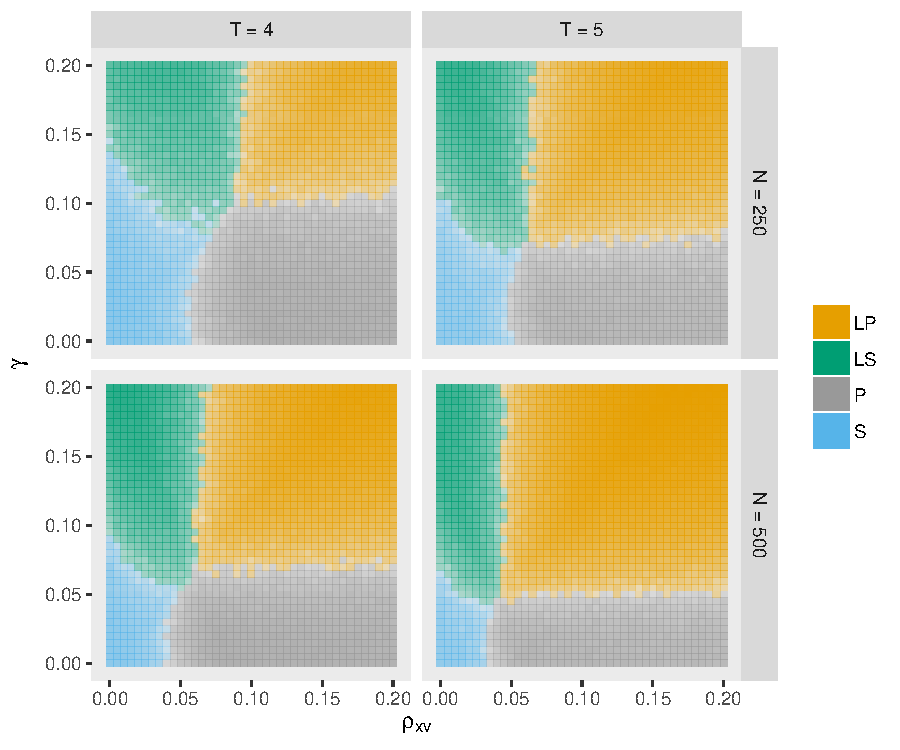
\includegraphics[scale = 0.8]{./simulations/DynamicPanel/results/Dpanel_oracle}
\caption{Minimum RMSE specification at each combination of parameter values for the simulation experiment from Section \ref{sec:Dpanel_sim_SR}. Color saturation at a given grid point indicates RMSE relative to second best specification.}
\label{fig:best}
\end{figure}
%%%%%%%%%%%%%%%%%%%%%%%%%%%%%%%%%%%%%%%%
\begin{sidewaystable}[htpb]
  \footnotesize
  \centering
  \begin{tabular}{cccc|cccc|cccc|cccc|cccc|cccc} 
 \hline \hline 
\multicolumn{4}{c}{}&\multicolumn{4}{c}{GFIC}&\multicolumn{4}{c}{LP}&\multicolumn{4}{c}{LS}&\multicolumn{4}{c}{P}&\multicolumn{4}{c}{S}\\ 
 \hline
 &  &  & $\rho$ & 0 & 0.05 & 0.1 & 0.15 & 0 & 0.05 & 0.1 & 0.15 & 0 & 0.05 & 0.1 & 0.15 & 0 & 0.05 & 0.1 & 0.15 & 0 & 0.05 & 0.1 & 0.15 \\
$T$ & $N$ & $\gamma$ &  &  &  &  &  &  &  &  &  &  &  &  &  &  &  &  &  &  &  &  &  \\
\hline
4 & 250 & 0 &  & 57 & 60 & 62 & 67 & 72 & 70 & 69 & 68 & 51 & 58 & 74 & 95 & 51 & 53 & 52 & 52 & 42 & 49 & 65 & 86 \\
 &  & 0.05 &  & 60 & 62 & 67 & 69 & 74 & 71 & 71 & 70 & 52 & 59 & 77 & 95 & 58 & 57 & 58 & 56 & 43 & 54 & 72 & 91 \\
 &  & 0.1 &  & 66 & 67 & 74 & 75 & 77 & 72 & 74 & 71 & 52 & 57 & 76 & 97 & 76 & 73 & 71 & 70 & 47 & 60 & 77 & 97 \\
 &  & 0.15 &  & 71 & 75 & 78 & 82 & 81 & 77 & 74 & 75 & 53 & 62 & 76 & 99 & 99 & 96 & 92 & 89 & 55 & 69 & 84 & 103 \\
 \hline
 & 500 & 0 &  & 40 & 43 & 48 & 48 & 51 & 49 & 49 & 48 & 37 & 47 & 67 & 90 & 37 & 37 & 36 & 36 & 30 & 40 & 59 & 83 \\
 &  & 0.05 &  & 43 & 47 & 51 & 49 & 52 & 50 & 51 & 49 & 36 & 47 & 67 & 90 & 45 & 45 & 44 & 43 & 31 & 47 & 65 & 87 \\
 &  & 0.1 &  & 45 & 53 & 56 & 54 & 52 & 51 & 50 & 50 & 36 & 47 & 69 & 90 & 67 & 64 & 62 & 59 & 37 & 53 & 73 & 92 \\
 &  & 0.15 &  & 50 & 56 & 59 & 56 & 56 & 53 & 52 & 50 & 36 & 48 & 69 & 92 & 92 & 90 & 85 & 83 & 45 & 63 & 80 & 100 \\
 \hline
5 & 250 & 0 &  & 45 & 48 & 54 & 56 & 56 & 56 & 55 & 54 & 42 & 51 & 70 & 91 & 44 & 45 & 44 & 45 & 36 & 44 & 62 & 83 \\
 &  & 0.05 &  & 48 & 52 & 56 & 55 & 58 & 56 & 55 & 54 & 43 & 52 & 70 & 92 & 52 & 51 & 51 & 48 & 38 & 50 & 68 & 89 \\
 &  & 0.1 &  & 51 & 57 & 61 & 58 & 59 & 57 & 55 & 55 & 44 & 53 & 72 & 94 & 68 & 66 & 65 & 62 & 42 & 57 & 75 & 95 \\
 &  & 0.15 &  & 55 & 61 & 65 & 64 & 60 & 60 & 58 & 57 & 44 & 52 & 74 & 94 & 94 & 89 & 85 & 81 & 51 & 64 & 83 & 100 \\
 \hline
 & 500 & 0 &  & 33 & 36 & 40 & 38 & 41 & 40 & 38 & 38 & 31 & 42 & 63 & 86 & 32 & 31 & 32 & 32 & 27 & 36 & 56 & 79 \\
 &  & 0.05 &  & 35 & 40 & 40 & 38 & 41 & 39 & 38 & 38 & 31 & 42 & 63 & 87 & 42 & 40 & 38 & 38 & 29 & 43 & 62 & 85 \\
 &  & 0.1 &  & 37 & 44 & 44 & 41 & 42 & 40 & 39 & 40 & 31 & 43 & 66 & 88 & 63 & 60 & 58 & 55 & 35 & 52 & 72 & 91 \\
 &  & 0.15 &  & 38 & 45 & 44 & 42 & 42 & 42 & 39 & 40 & 31 & 44 & 67 & 90 & 88 & 85 & 80 & 76 & 44 & 62 & 80 & 98 \\
\hline
\end{tabular}


  \vspace{2em}
  \begin{tabular}{cccc|cccc|cccc|cccc|cccc|cccc} 
 \hline \hline 
\multicolumn{4}{c}{}&\multicolumn{4}{c}{Oracle}&\multicolumn{4}{c}{GFIC}&\multicolumn{4}{c}{J-test 5\%}&\multicolumn{4}{c}{GMM-BIC}&\multicolumn{4}{c}{GMM-AIC}\\ 
 \hline
 &  &  & $\rho$ & 0 & 0.05 & 0.1 & 0.15 & 0 & 0.05 & 0.1 & 0.15 & 0 & 0.05 & 0.1 & 0.15 & 0 & 0.05 & 0.1 & 0.15 & 0 & 0.05 & 0.1 & 0.15 \\
$T$ & $N$ & $\gamma$ &  &  &  &  &  &  &  &  &  &  &  &  &  &  &  &  &  &  &  &  &  \\
4 & 250 & 0 &  & 42 & 49 & 52 & 52 & 57 & 60 & 62 & 67 & 44 & 52 & 66 & 80 & 44 & 51 & 68 & 89 & 52 & 58 & 72 & 81 \\
 &  & 0.05 &  & 43 & 54 & 58 & 56 & 60 & 62 & 67 & 69 & 47 & 55 & 72 & 88 & 46 & 55 & 73 & 93 & 53 & 60 & 75 & 88 \\
 &  & 0.1 &  & 47 & 57 & 71 & 70 & 66 & 67 & 74 & 75 & 55 & 61 & 78 & 95 & 50 & 60 & 78 & 98 & 59 & 64 & 79 & 92 \\
 &  & 0.15 &  & 53 & 62 & 74 & 75 & 71 & 75 & 78 & 82 & 68 & 74 & 86 & 102 & 57 & 69 & 83 & 103 & 66 & 73 & 84 & 100 \\
 & 500 & 0 &  & 30 & 37 & 36 & 36 & 40 & 43 & 48 & 48 & 32 & 41 & 55 & 61 & 31 & 42 & 61 & 85 & 37 & 47 & 58 & 61 \\
 &  & 0.05 &  & 31 & 45 & 44 & 43 & 43 & 47 & 51 & 49 & 34 & 47 & 64 & 74 & 32 & 47 & 66 & 88 & 39 & 49 & 64 & 67 \\
 &  & 0.1 &  & 36 & 47 & 50 & 50 & 45 & 53 & 56 & 54 & 46 & 55 & 71 & 86 & 39 & 53 & 73 & 92 & 44 & 54 & 70 & 78 \\
 &  & 0.15 &  & 36 & 48 & 52 & 50 & 50 & 56 & 59 & 56 & 68 & 67 & 81 & 97 & 43 & 62 & 80 & 100 & 52 & 61 & 78 & 92 \\
5 & 250 & 0 &  & 36 & 44 & 44 & 45 & 45 & 48 & 54 & 56 & 37 & 45 & 62 & 74 & 40 & 49 & 68 & 89 & 43 & 50 & 66 & 75 \\
 &  & 0.05 &  & 38 & 50 & 51 & 48 & 48 & 52 & 56 & 55 & 41 & 51 & 67 & 82 & 42 & 52 & 70 & 92 & 44 & 54 & 68 & 79 \\
 &  & 0.1 &  & 42 & 53 & 55 & 55 & 51 & 57 & 61 & 58 & 47 & 58 & 74 & 91 & 44 & 56 & 74 & 95 & 48 & 58 & 73 & 87 \\
 &  & 0.15 &  & 44 & 52 & 58 & 57 & 55 & 61 & 65 & 64 & 63 & 67 & 82 & 97 & 46 & 58 & 80 & 99 & 54 & 61 & 79 & 93 \\
 & 500 & 0 &  & 27 & 31 & 32 & 32 & 33 & 36 & 40 & 38 & 28 & 37 & 51 & 51 & 30 & 41 & 62 & 84 & 31 & 41 & 53 & 50 \\
 &  & 0.05 &  & 29 & 39 & 38 & 38 & 35 & 40 & 40 & 38 & 31 & 44 & 59 & 66 & 31 & 44 & 64 & 86 & 33 & 44 & 57 & 56 \\
 &  & 0.1 &  & 31 & 40 & 39 & 40 & 37 & 44 & 44 & 41 & 41 & 52 & 70 & 83 & 32 & 48 & 71 & 90 & 37 & 49 & 66 & 70 \\
 &  & 0.15 &  & 31 & 42 & 39 & 40 & 38 & 45 & 44 & 42 & 65 & 65 & 79 & 94 & 33 & 52 & 76 & 96 & 41 & 55 & 73 & 84 \\
\hline
\end{tabular}
  \caption{RMSE values multiplied by 1000 for the simulation experiment from Section \ref{sec:Dpanel_sim_SR}.}
  \label{tab:Dpanel_RMSE}
\end{sidewaystable}
%%%%%%%%%%%%%%%%%%%%%%%%%%%%%%%%%%%%%%%%

In practice, of course, we do not know the values of $\gamma$, $\rho$, $\theta$, or the other parameters of the DGP so this comparison of finite-sample RMSE values is infeasible.
Instead, we consider using the GFIC to select between the four specifications.
Clearly there are gains to be had from estimating a mis-specified model in certain situations.
The questions remains, can the GFIC identify them?
Because it is an efficient rather than consistent selection criterion, the GFIC remains random, even in the limit.
This means that the GFIC can never outperform the ``oracle'' estimator that uses whichever specification gives the lowest finite-sample RMSE in figure \ref{fig:best}.
Moreover, because our target parameter is a scalar, Stein-type results do not apply: the post-GFIC estimator cannot provide a uniform improvement over the true specification $\text{LP}$.
Nevertheless, the post-GFIC estimator can provide a substantial improvement over $\text{LP}$ when $\rho_{xv}$ and $\gamma$ are relatively small relative to sample size, as shown in Figure \ref{fig:GFIC_rel_LP} and in the two leftmost panes of the top panel in Table \ref{tab:Dpanel_RMSE}.
This is precisely the situation for which the GFIC is intended: a setting in which we have reason to suspect that mis-specification is fairly mild.
Moreover, in situations where $\text{LP}$ has a substantially lower RMSE than the other estimators, the post GFIC-estimator's performance is comparable.

%%%%%%%%%%%%%%%%%%%%%%%%%%%%%%%%%%%%%%%%
\begin{figure}
\centering
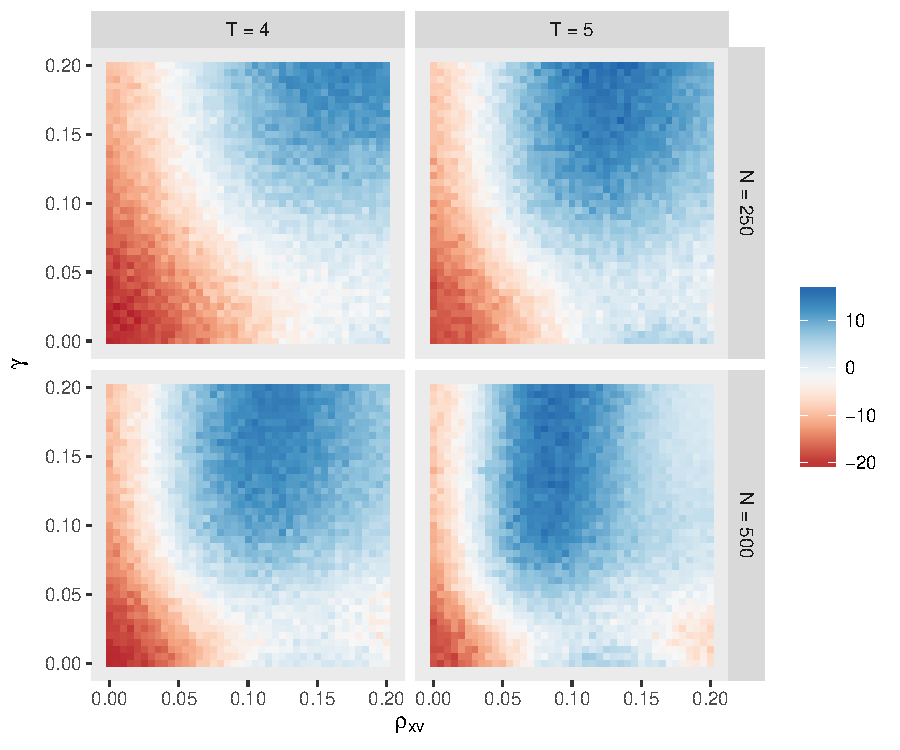
\includegraphics[scale = 0.8]{./simulations/DynamicPanel/results/Dpanel_GFIC_RMSE_rel_LP}
\caption{RMSE of the post-GFIC estimator relative to that of the true specification ($\text{LP}$) in the dynamic panel simulation experiment from Section \ref{sec:Dpanel_sim_SR}.}
\label{fig:GFIC_rel_LP}
\end{figure}
%%%%%%%%%%%%%%%%%%%%%%%%%%%%%%%%%%%%%%%%

To provide a basis for comparison, we now consider results for a number of alternative selection procedures. 
The first is a ``Downward J-test,'' which is intended to approximate what applied researchers may do in practice when faced with a model and moment selection decision such as this one.
The Downward J-test selects the \emph{most restrictive} specification that is not rejected by a J-test test with significance level $\alpha \in \left\{ 0.05, 0.1 \right\}$.
We test the specifications $\left\{\text{S}, \text{P}, \text{LS}, \text{LP}\right\}$ \emph{in order} and report the first that is \emph{not rejected}.
This means that we only report $\text{LP}$ if all the other specifications have been rejected.
This procedure is, of course, somewhat \emph{ad hoc} because the significance threshold $\alpha$ is chosen arbitrarily rather than with a view towards some kind of selection optimality. 
We also consider the GMM model and moment selection criteria of \cite{AndrewsLu}: 
	\begin{align*}
	 \mbox{GMM-BIC} &= J - (|c| - |b|) \log{n}\\
	 \mbox{GMM-AIC}&= J - 2(|c| - |b|)\\ 
	 \mbox{GMM-HQ} &= J - 2.01 (|c| - |b|)  \log{\log{n}}
	\end{align*}
where $|b|$ is the number of parameters estimated, and $|c|$ the number of moment conditions used. 
Under certain assumptions, it can be shown that both the GMM-BIC and GMM-HQ are consistent: they select the maximal correctly specified estimator with probability approaching one in the limit. 
To implement these criteria, we calculate the J-test based on the optimal, two-step GMM estimator with a panel robust, heteroscedasticity-consistent, centered covariance matrix estimator for each specification.
To compare selection procedures we use the same simulation grid as above, namely $\gamma$ and $\sigma_{xv}$, namely $\gamma, \sigma_{xv} \in \{0, 0.005, 0.01, \hdots, 0.195, 0.20\}$.  
Again, each point on the simulation grid is calculated from 2000 simulation replications. 
The bottom panel of Table \ref{tab:Dpanel_RMSE} presents results for these alternative selection procedures.
Figures comparing the GFIC against each alternative in turn appear in Appendix \ref{sec:simulation_supplement}.
There is no clear winner in point-wise RMSE comparisons between the GFIC and its competitors. 
A substantial difference between the GFIC and its competitors emerges, however, when we examine worst-case RMSE.
Here the GFIC clearly dominates, providing the lowest worst-case RMSE across all configurations of $T$ and $n$.
The differences are particularly stark for larger sample sizes.
For example, when $T=5$ and $n=500$ the worst-case RMSE of GFIC is approximately half that of its nearest competitor: GMM-AIC.
The consistent criteria, GMM-BIC and GMM-HQ, perform particularly poorly in terms of worst-case RMSE.
This is unsurprising given that the worst-case risk of any consistent selection criteria diverges as sample size increases.\footnote{See, e.g., \cite{LeebPoetscher2008}.}

\subsection{Slope Heterogeneity Example}
In the interest of space we omit the simulation results for the slope heterogeneity example from Section \ref{sec:slopeHet}.
These are available upon request.
